\subsection{Mean model == Mean measurement?}
For a selection of three model measurements:

Over rheobase, input resistance, capacitance, and time constant, we took measurements by instancing two different models at  two different loctations in parameter space. With these two different models we took seperate measurements of all the appropriate model properties, then we averaged these measurements together, to get the 'mean measurements', secondly we created a 'mean model' by averaging the two points together in parameter space and instancing the 'mean parameter model'. We then used the mean model to create a third set of measurements.

When we have mean measurements, and also mean model measurements, it enables us to understand if bi-modal distributions of measurements in experimental data can pose a problem for optimization of cells.

Previously in methods \ref{section:nelectro} , we graphically inspected the neuroelectro data sources closely, in order to assess each measurements distribution. We revealed Bi-modal distributions in input resistance, and cell membrane capacitance, but we do not yet know if it is invalid to fit to the mean of a bi-modal distribution. Consider a  cell class which had an underlying bimodal distribution for input resistance. An individual cell from this class produced measurements for input resistance midway between two modes for input resistance. Its entirely concievable that that this mean cell would produce measurements that were also the mean of the two modes, however, we cannot assume that there this to be true, it seems equally likely that this midway cell produces a measurement for input resistance, that is significantly higher or lower than the mean of the two modes. To bolster that this non linear behavior could be a problem with in-silico models of in-vivo experiments. We created virtual experiments to expose non-linear behavior between two  close, but different sets of model parameters.

%set about establishing that it is a problem in modelling space.
%The genetic algorithm approach, of recombining model parameters to sample error surface is a similar concept. We do not naively interpolate using midway points, becuase we don't expect that small changes in model parameters to have linear effects.
%to sampling models 

We expect the Izhikitich model, and the adaptive exponential models to support "regime" change, that is we know that there are regions in parameter space that where when entered cell behavior becomes fundamentally different. For instance in the Izhikevich model, some regions support tonic-bursting and other regions support chattering. 

\begin{figure}
    \centering
    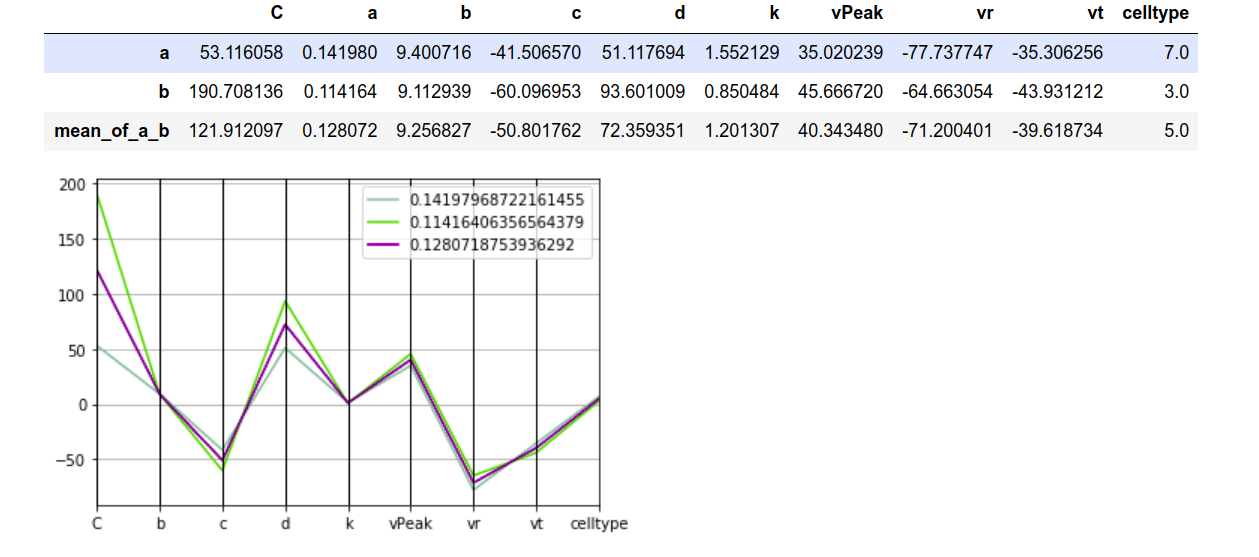
\includegraphics{figures/mean_model_mean_measure_ment_params.png}
    \caption{Caption}
    \label{fig:my_label}
\end{figure}

\begin{figure}
    \centering
    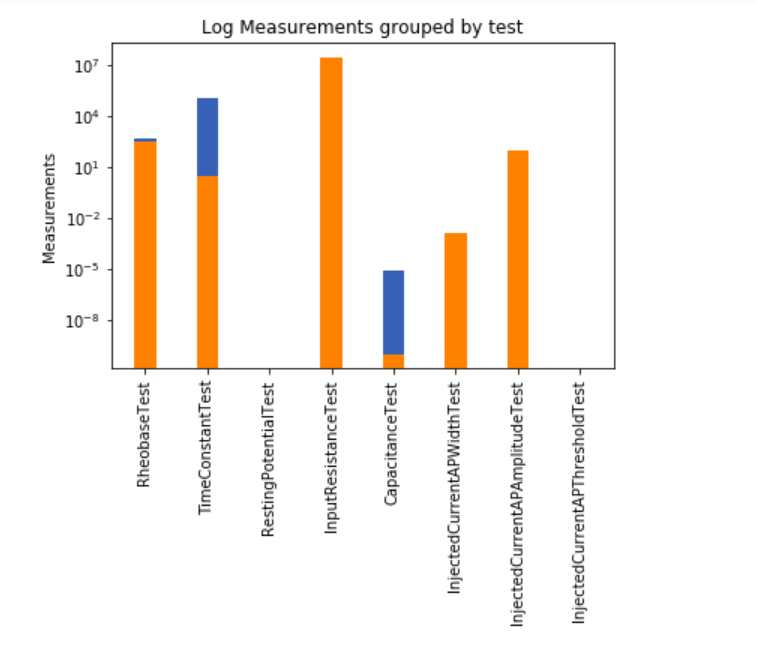
\includegraphics{figures/mean_model_mean_test.png}
    \caption{Caption}
    \label{fig:my_label}
\end{figure}

\begin{figure}
    \centering
    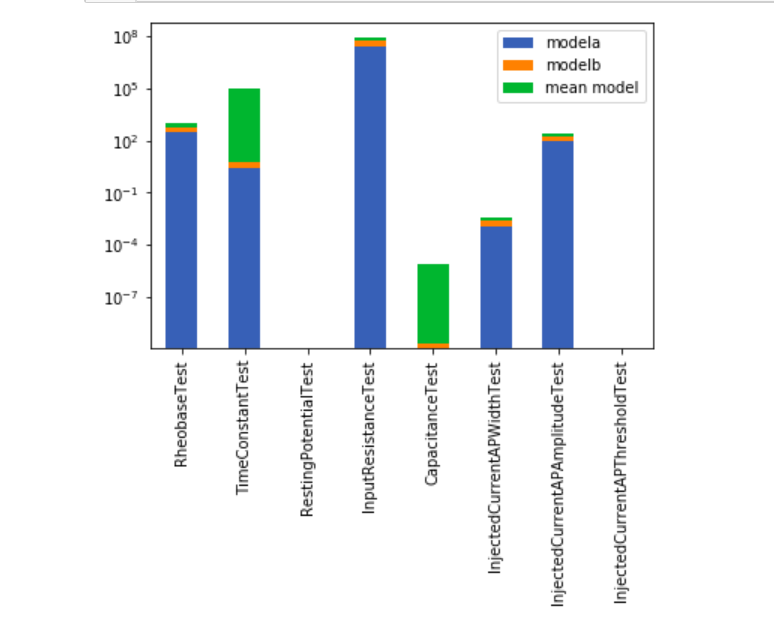
\includegraphics{figures/mean_model_mean_test2.png}
    \caption{Caption}
    \label{fig:my_label}
\end{figure}

explore if this was a problem for models as well as experimental cells.